\documentclass[11pt]{article}
\usepackage[textwidth=18.0cm, textheight=23.0cm, top=2.0cm]{geometry}
\usepackage{pst-all}
\usepackage{amssymb}
\usepackage{tikz}
\usepackage{underscore}\begin{document}
\pagestyle{empty}


ClassName: \underline{\textbf{Class_03.2bp-22}}
\par
BinSize: \underline{\textbf{40 × 40}}
\par
ReduceSize: \underline{\textbf{40 × 40}}
\par
TypeNum: \underline{\textbf{60}}
\par
Num: \underline{\textbf{60}}
\par
OutS: \underline{\textbf{22400}}
\par
InS: \underline{\textbf{19664}}
\par
Rate: \underline{\textbf{0.878}}
\par
UB: \underline{\textbf{14}}
\par
LB0: \underline{\textbf{13}}
\par
LB: \underline{\textbf{14}}
\par
LBWithCut: \underline{\textbf{14}}
\par
NodeCut: \underline{\textbf{0}}
\par
ExtendedNodeCnt: \underline{\textbf{1}}
\par
GenNodeCnt: \underline{\textbf{1}}
\par
PrimalNode: \underline{\textbf{0}}
\par
ColumnCount: \underline{\textbf{184}}
\par
TotalCutCount: \underline{\textbf{0}}
\par
RootCutCount: \underline{\textbf{0}}
\par
LPSolverCnt: \underline{\textbf{171}}
\par
PricingSolverCnt: \underline{\textbf{171}}
\par
BranchAndBoundNum: \underline{\textbf{1}}
\par
isOpt: \underline{\textbf{true}}
\par
TimeOnInitSolution: \underline{\textbf{600.000 s}}
\par
TimeOnPrimal: \underline{\textbf{0.000 s}}
\par
TimeOnPricing: \underline{\textbf{127.865 s}}
\par
TimeOnRmp: \underline{\textbf{0.145 s}}
\par
TotalTime: \underline{\textbf{728.309 s}}
\par
\newpage


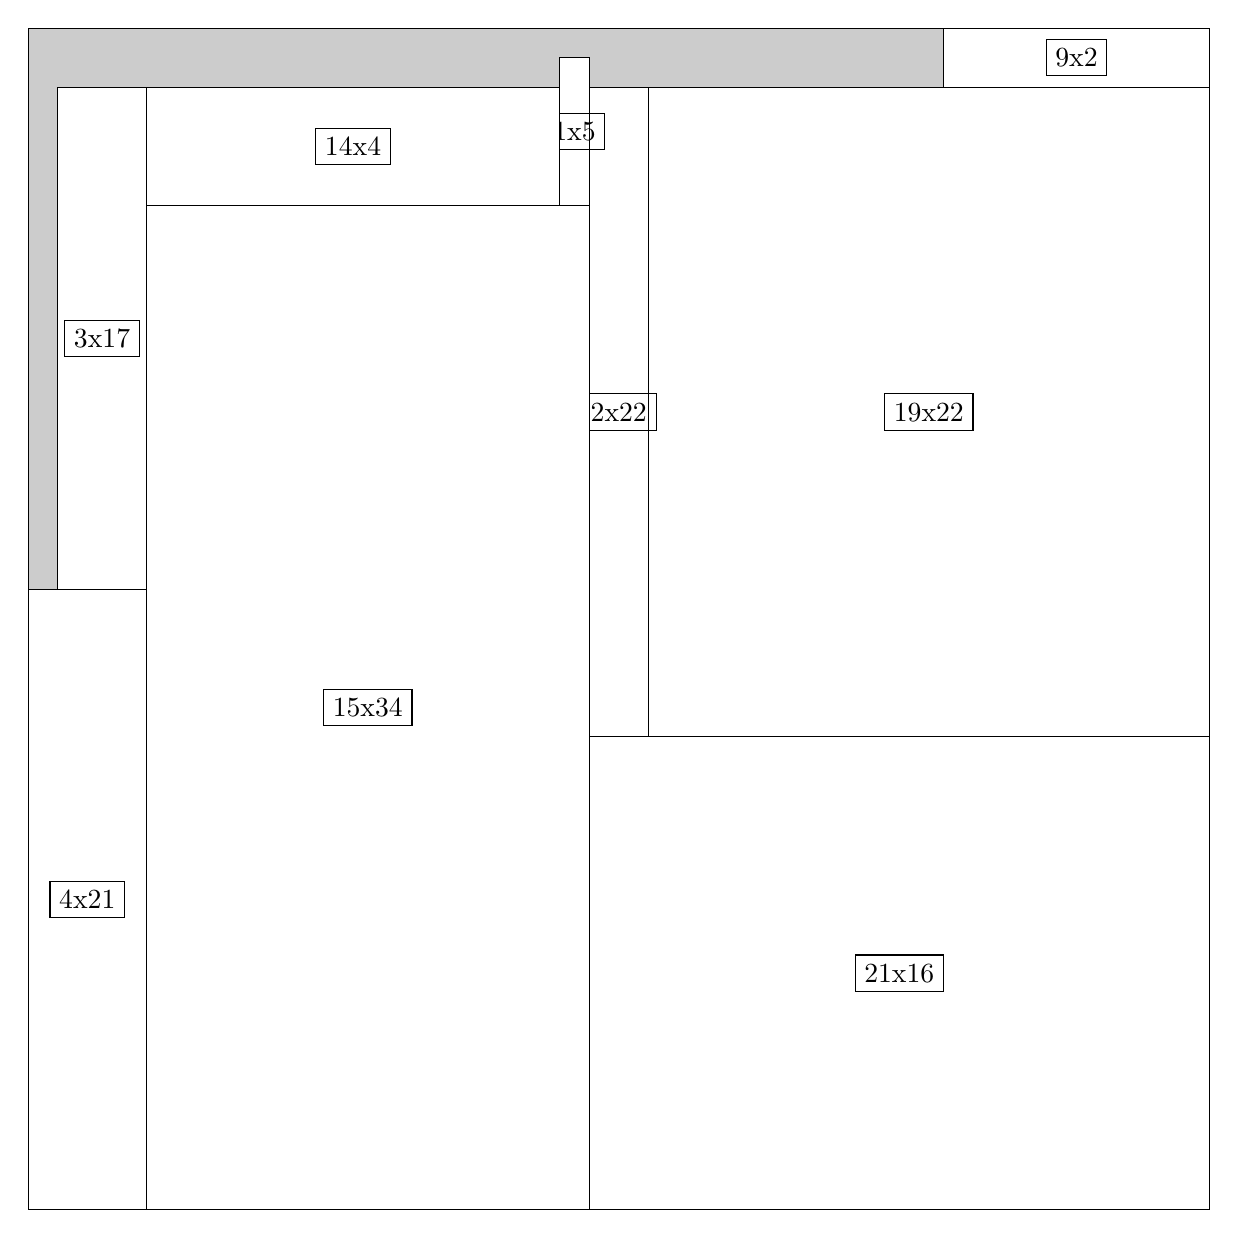
\begin{tikzpicture}[shorten >=1pt,scale=1.0,every node/.style={scale=1.0},->]
\tikzstyle{vertex}=[circle,fill=black!25,minimum size=14pt,inner sep=0pt]
\filldraw[fill=gray!40!white, draw=black] (0,0) rectangle (15.0,15.0);
\foreach \name/\x/\y/\w/\h in {21x16/7.125/0.0/7.875/6.0,19x22/7.875/6.0/7.125/8.25,9x2/11.625/14.25/3.375/0.75,2x22/7.125/6.0/0.75/8.25,15x34/1.5/0.0/5.625/12.75,1x5/6.75/12.75/0.375/1.875,14x4/1.5/12.75/5.25/1.5,4x21/0.0/0.0/1.5/7.875,3x17/0.375/7.875/1.125/6.375}
\filldraw[fill=white!40!white, draw=black] (\x,\y) rectangle node[draw] (\name) {\name} ++(\w,\h);
\end{tikzpicture}


w =21 , h =16 , x =19 , y =0 , v =336
\par
w =19 , h =22 , x =21 , y =16 , v =418
\par
w =9 , h =2 , x =31 , y =38 , v =18
\par
w =2 , h =22 , x =19 , y =16 , v =44
\par
w =15 , h =34 , x =4 , y =0 , v =510
\par
w =1 , h =5 , x =18 , y =34 , v =5
\par
w =14 , h =4 , x =4 , y =34 , v =56
\par
w =4 , h =21 , x =0 , y =0 , v =84
\par
w =3 , h =17 , x =1 , y =21 , v =51
\par
\newpage


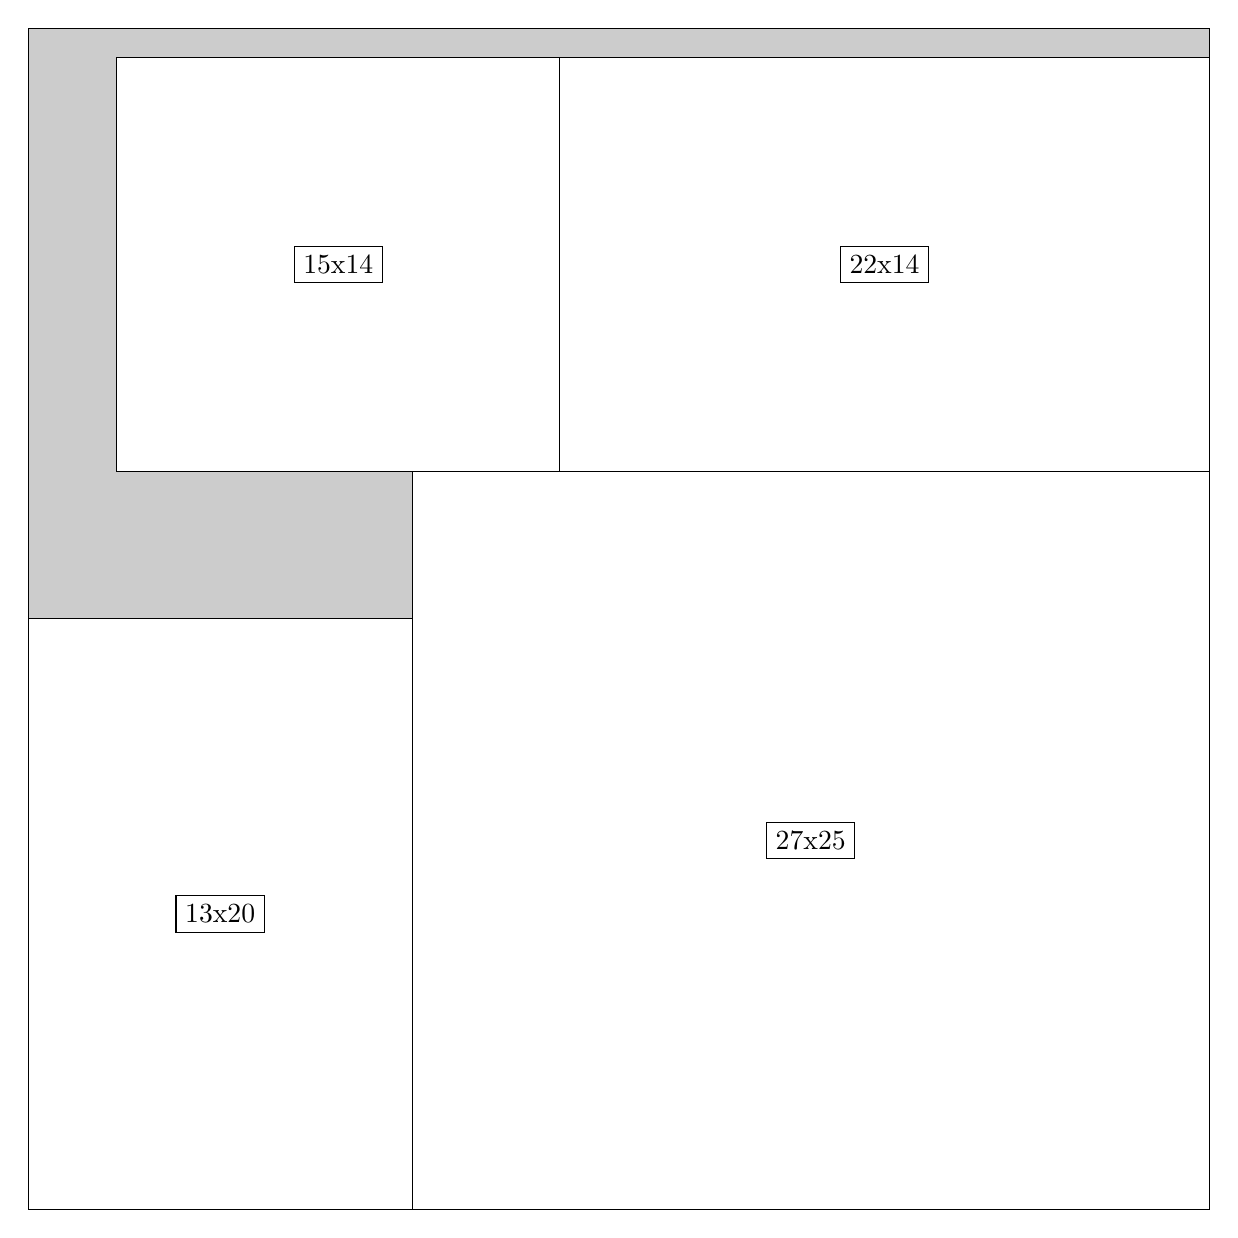
\begin{tikzpicture}[shorten >=1pt,scale=1.0,every node/.style={scale=1.0},->]
\tikzstyle{vertex}=[circle,fill=black!25,minimum size=14pt,inner sep=0pt]
\filldraw[fill=gray!40!white, draw=black] (0,0) rectangle (15.0,15.0);
\foreach \name/\x/\y/\w/\h in {27x25/4.875/0.0/10.125/9.375,13x20/0.0/0.0/4.875/7.5,22x14/6.75/9.375/8.25/5.25,15x14/1.125/9.375/5.625/5.25}
\filldraw[fill=white!40!white, draw=black] (\x,\y) rectangle node[draw] (\name) {\name} ++(\w,\h);
\end{tikzpicture}


w =27 , h =25 , x =13 , y =0 , v =675
\par
w =13 , h =20 , x =0 , y =0 , v =260
\par
w =22 , h =14 , x =18 , y =25 , v =308
\par
w =15 , h =14 , x =3 , y =25 , v =210
\par
\newpage


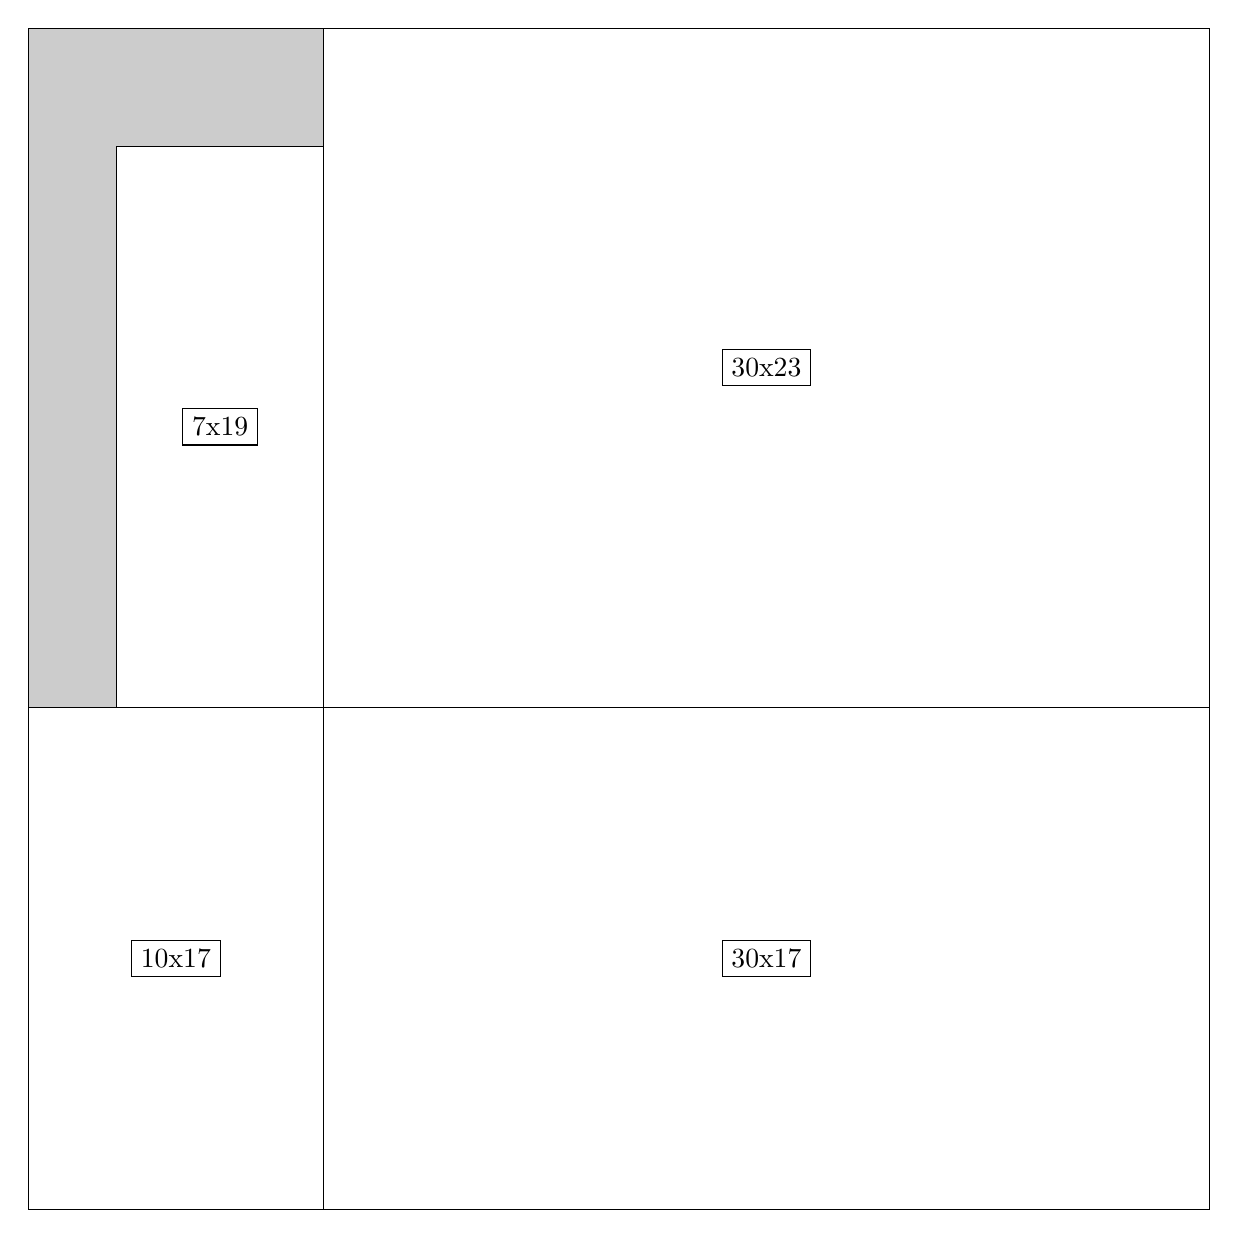
\begin{tikzpicture}[shorten >=1pt,scale=1.0,every node/.style={scale=1.0},->]
\tikzstyle{vertex}=[circle,fill=black!25,minimum size=14pt,inner sep=0pt]
\filldraw[fill=gray!40!white, draw=black] (0,0) rectangle (15.0,15.0);
\foreach \name/\x/\y/\w/\h in {30x17/3.75/0.0/11.25/6.375,10x17/0.0/0.0/3.75/6.375,30x23/3.75/6.375/11.25/8.625,7x19/1.125/6.375/2.625/7.125}
\filldraw[fill=white!40!white, draw=black] (\x,\y) rectangle node[draw] (\name) {\name} ++(\w,\h);
\end{tikzpicture}


w =30 , h =17 , x =10 , y =0 , v =510
\par
w =10 , h =17 , x =0 , y =0 , v =170
\par
w =30 , h =23 , x =10 , y =17 , v =690
\par
w =7 , h =19 , x =3 , y =17 , v =133
\par
\newpage


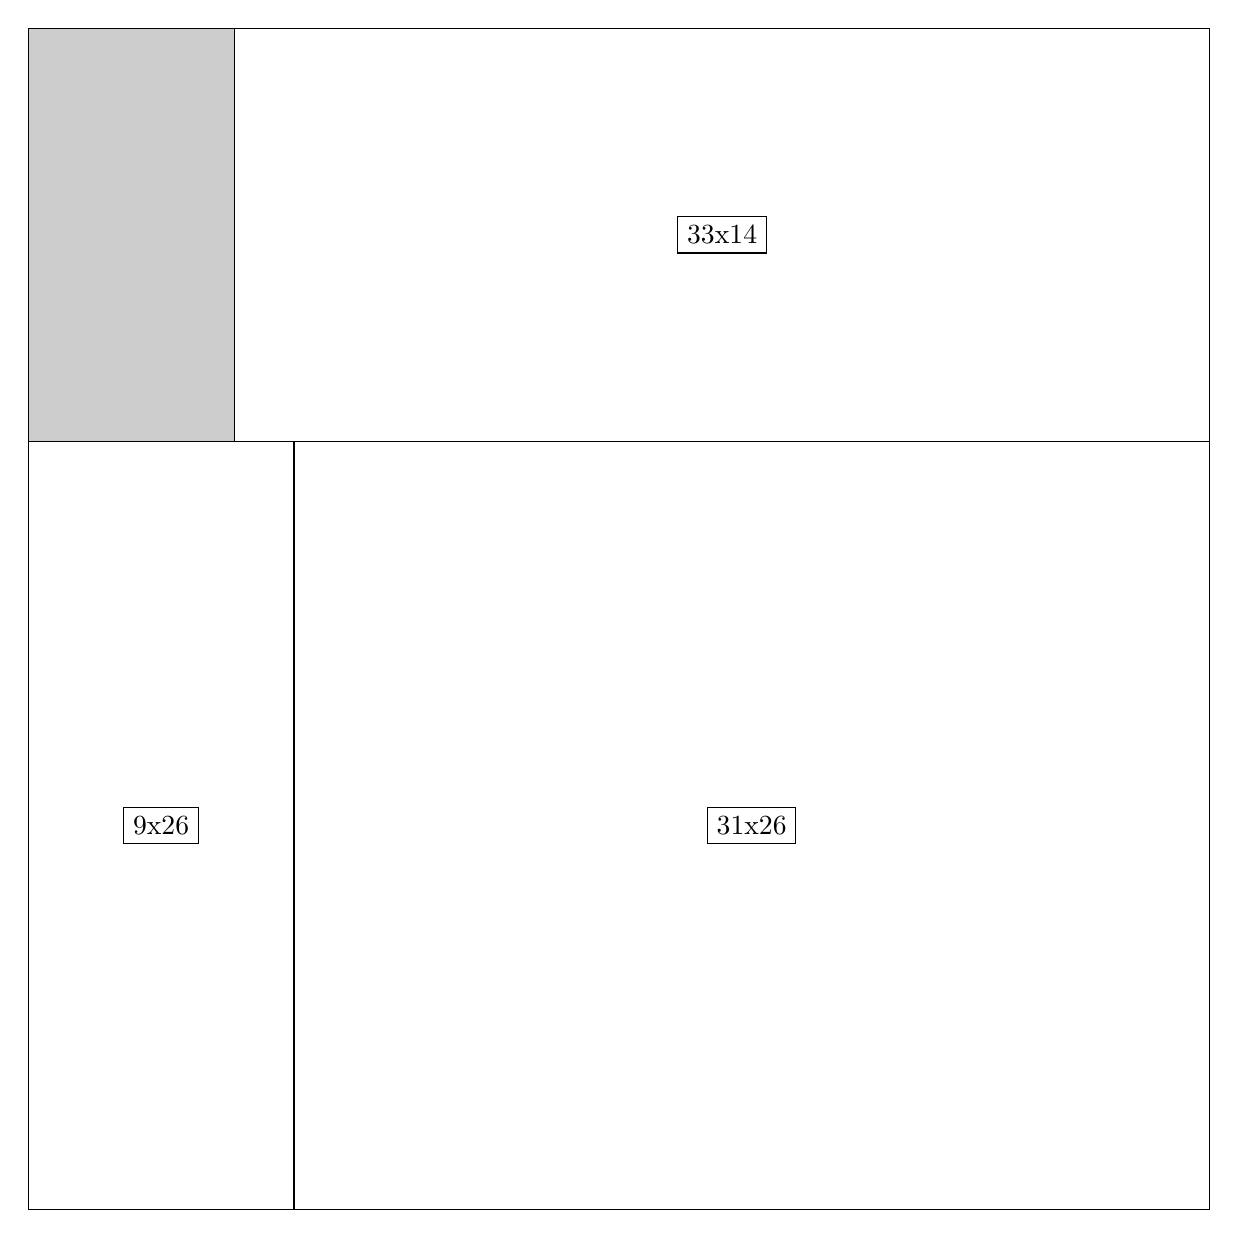
\begin{tikzpicture}[shorten >=1pt,scale=1.0,every node/.style={scale=1.0},->]
\tikzstyle{vertex}=[circle,fill=black!25,minimum size=14pt,inner sep=0pt]
\filldraw[fill=gray!40!white, draw=black] (0,0) rectangle (15.0,15.0);
\foreach \name/\x/\y/\w/\h in {31x26/3.375/0.0/11.625/9.75,9x26/0.0/0.0/3.375/9.75,33x14/2.625/9.75/12.375/5.25}
\filldraw[fill=white!40!white, draw=black] (\x,\y) rectangle node[draw] (\name) {\name} ++(\w,\h);
\end{tikzpicture}


w =31 , h =26 , x =9 , y =0 , v =806
\par
w =9 , h =26 , x =0 , y =0 , v =234
\par
w =33 , h =14 , x =7 , y =26 , v =462
\par
\newpage


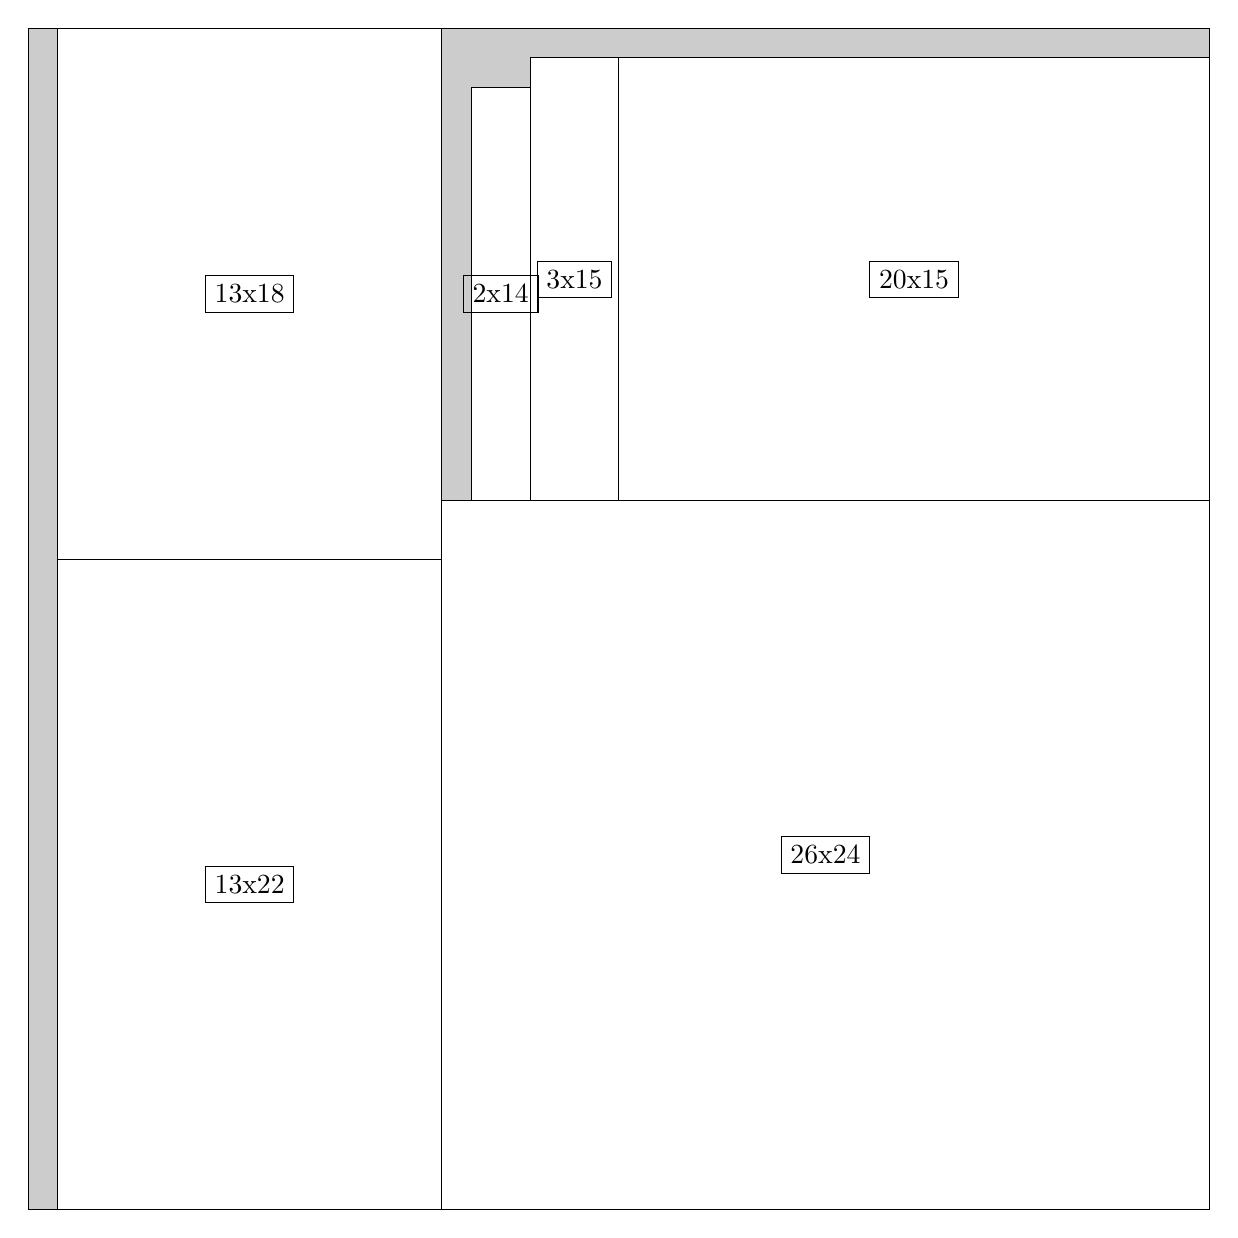
\begin{tikzpicture}[shorten >=1pt,scale=1.0,every node/.style={scale=1.0},->]
\tikzstyle{vertex}=[circle,fill=black!25,minimum size=14pt,inner sep=0pt]
\filldraw[fill=gray!40!white, draw=black] (0,0) rectangle (15.0,15.0);
\foreach \name/\x/\y/\w/\h in {26x24/5.25/0.0/9.75/9.0,20x15/7.5/9.0/7.5/5.625,3x15/6.375/9.0/1.125/5.625,2x14/5.625/9.0/0.75/5.25,13x22/0.375/0.0/4.875/8.25,13x18/0.375/8.25/4.875/6.75}
\filldraw[fill=white!40!white, draw=black] (\x,\y) rectangle node[draw] (\name) {\name} ++(\w,\h);
\end{tikzpicture}


w =26 , h =24 , x =14 , y =0 , v =624
\par
w =20 , h =15 , x =20 , y =24 , v =300
\par
w =3 , h =15 , x =17 , y =24 , v =45
\par
w =2 , h =14 , x =15 , y =24 , v =28
\par
w =13 , h =22 , x =1 , y =0 , v =286
\par
w =13 , h =18 , x =1 , y =22 , v =234
\par
\newpage


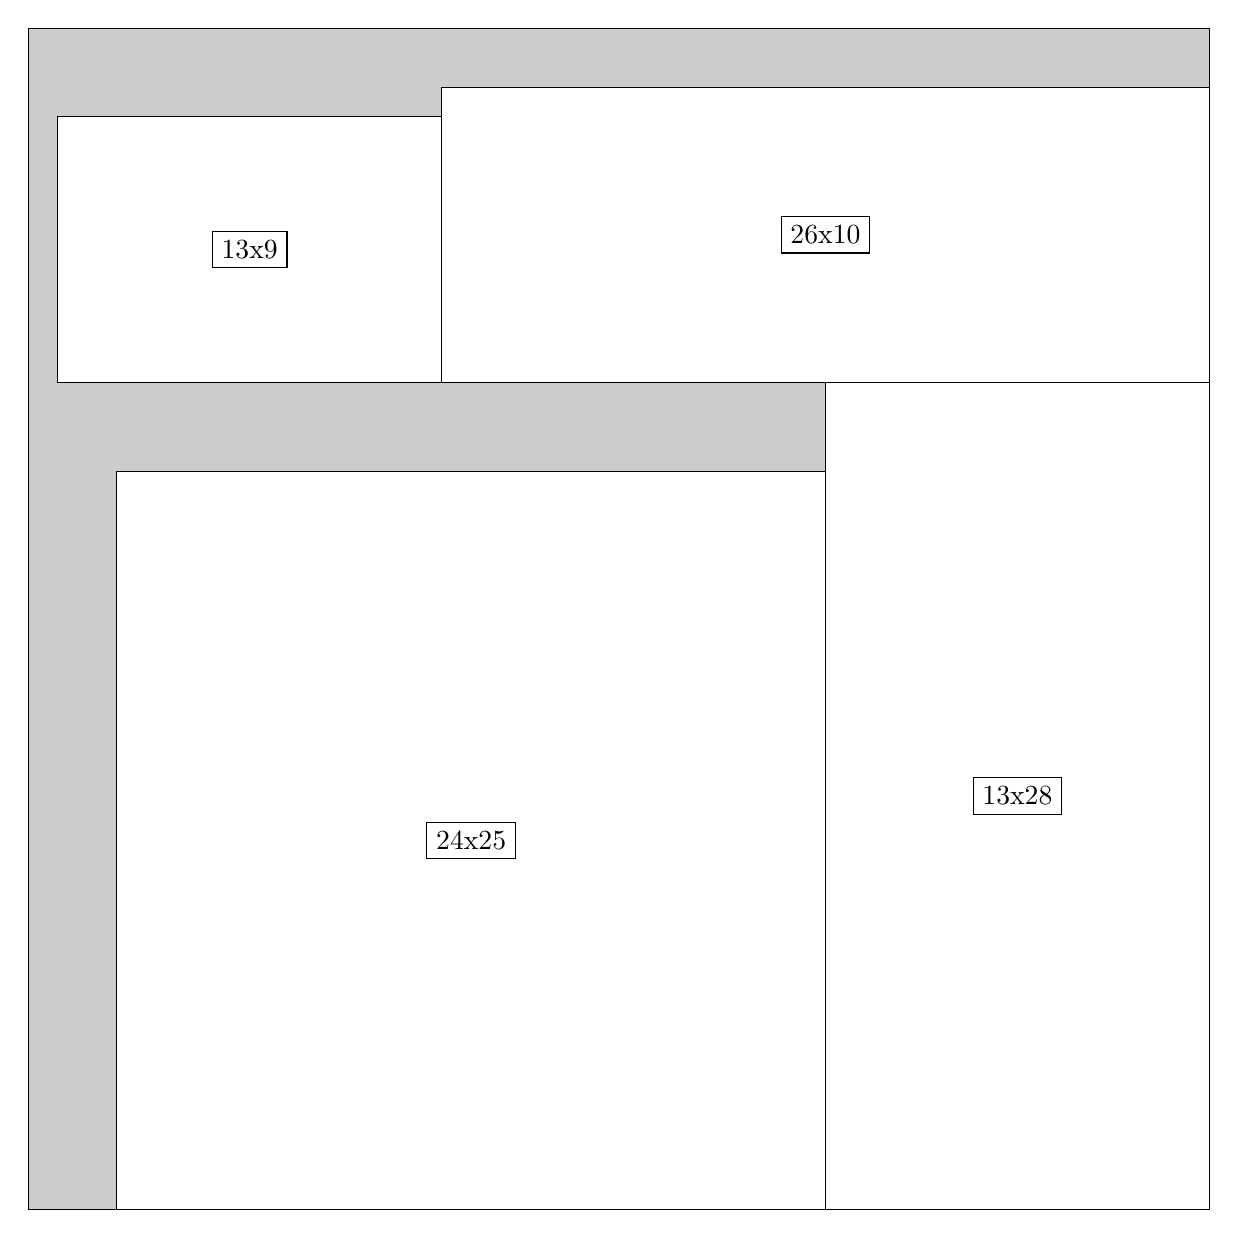
\begin{tikzpicture}[shorten >=1pt,scale=1.0,every node/.style={scale=1.0},->]
\tikzstyle{vertex}=[circle,fill=black!25,minimum size=14pt,inner sep=0pt]
\filldraw[fill=gray!40!white, draw=black] (0,0) rectangle (15.0,15.0);
\foreach \name/\x/\y/\w/\h in {13x28/10.125/0.0/4.875/10.5,24x25/1.125/0.0/9.0/9.375,26x10/5.25/10.5/9.75/3.75,13x9/0.375/10.5/4.875/3.375}
\filldraw[fill=white!40!white, draw=black] (\x,\y) rectangle node[draw] (\name) {\name} ++(\w,\h);
\end{tikzpicture}


w =13 , h =28 , x =27 , y =0 , v =364
\par
w =24 , h =25 , x =3 , y =0 , v =600
\par
w =26 , h =10 , x =14 , y =28 , v =260
\par
w =13 , h =9 , x =1 , y =28 , v =117
\par
\newpage


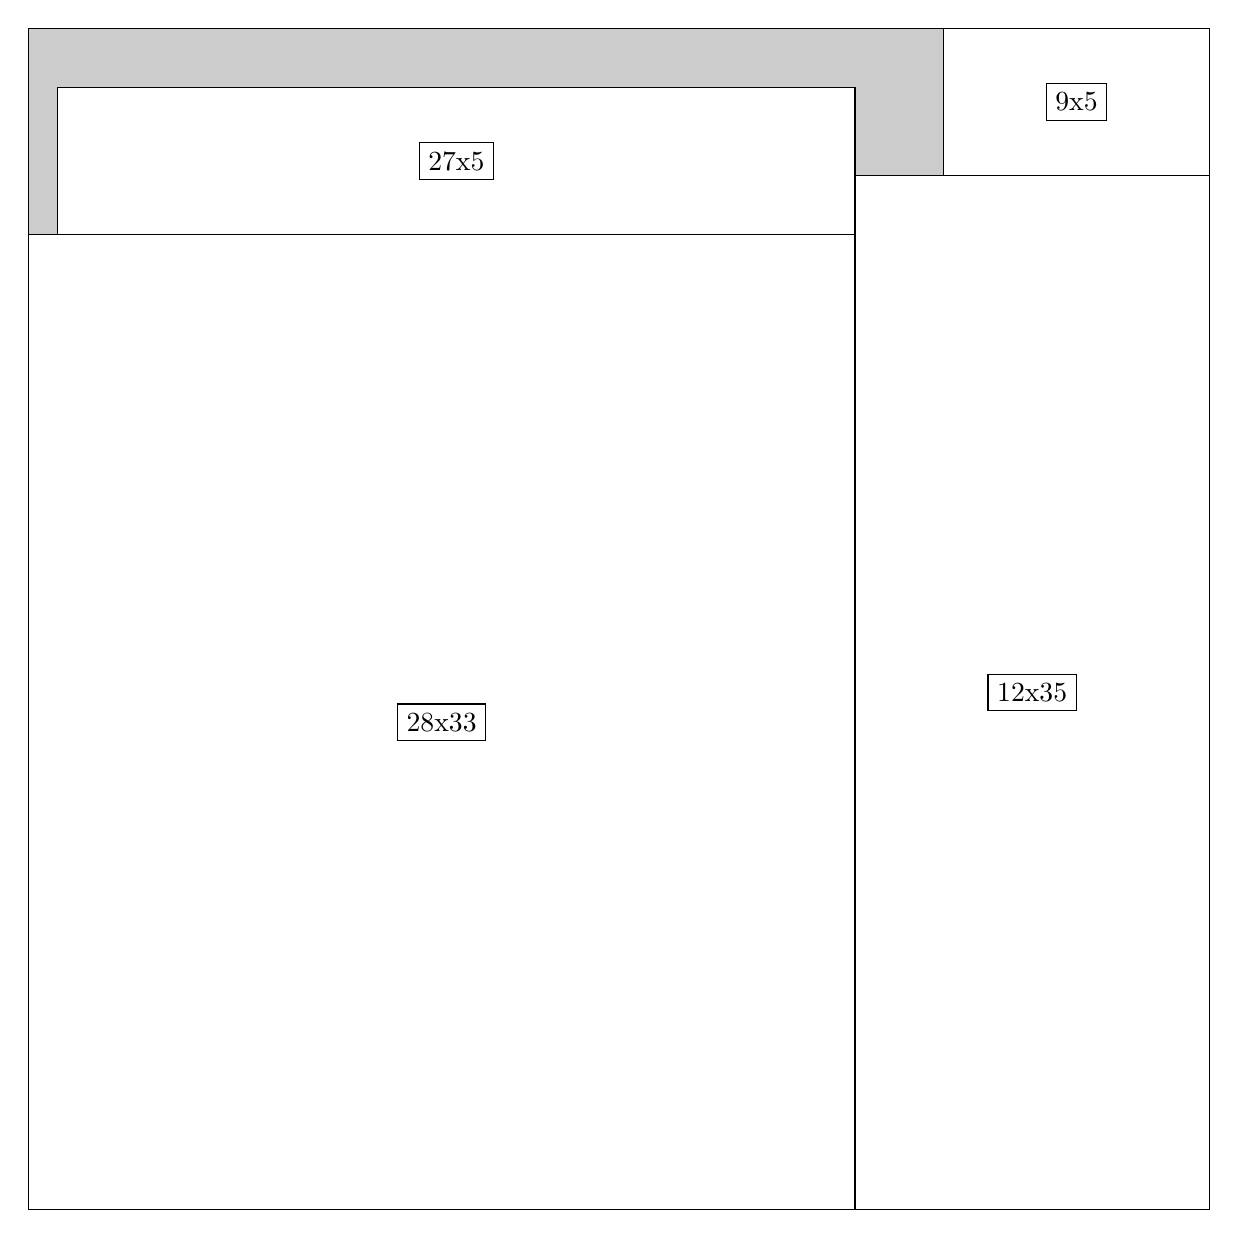
\begin{tikzpicture}[shorten >=1pt,scale=1.0,every node/.style={scale=1.0},->]
\tikzstyle{vertex}=[circle,fill=black!25,minimum size=14pt,inner sep=0pt]
\filldraw[fill=gray!40!white, draw=black] (0,0) rectangle (15.0,15.0);
\foreach \name/\x/\y/\w/\h in {12x35/10.5/0.0/4.5/13.125,9x5/11.625/13.125/3.375/1.875,28x33/0.0/0.0/10.5/12.375,27x5/0.375/12.375/10.125/1.875}
\filldraw[fill=white!40!white, draw=black] (\x,\y) rectangle node[draw] (\name) {\name} ++(\w,\h);
\end{tikzpicture}


w =12 , h =35 , x =28 , y =0 , v =420
\par
w =9 , h =5 , x =31 , y =35 , v =45
\par
w =28 , h =33 , x =0 , y =0 , v =924
\par
w =27 , h =5 , x =1 , y =33 , v =135
\par
\newpage


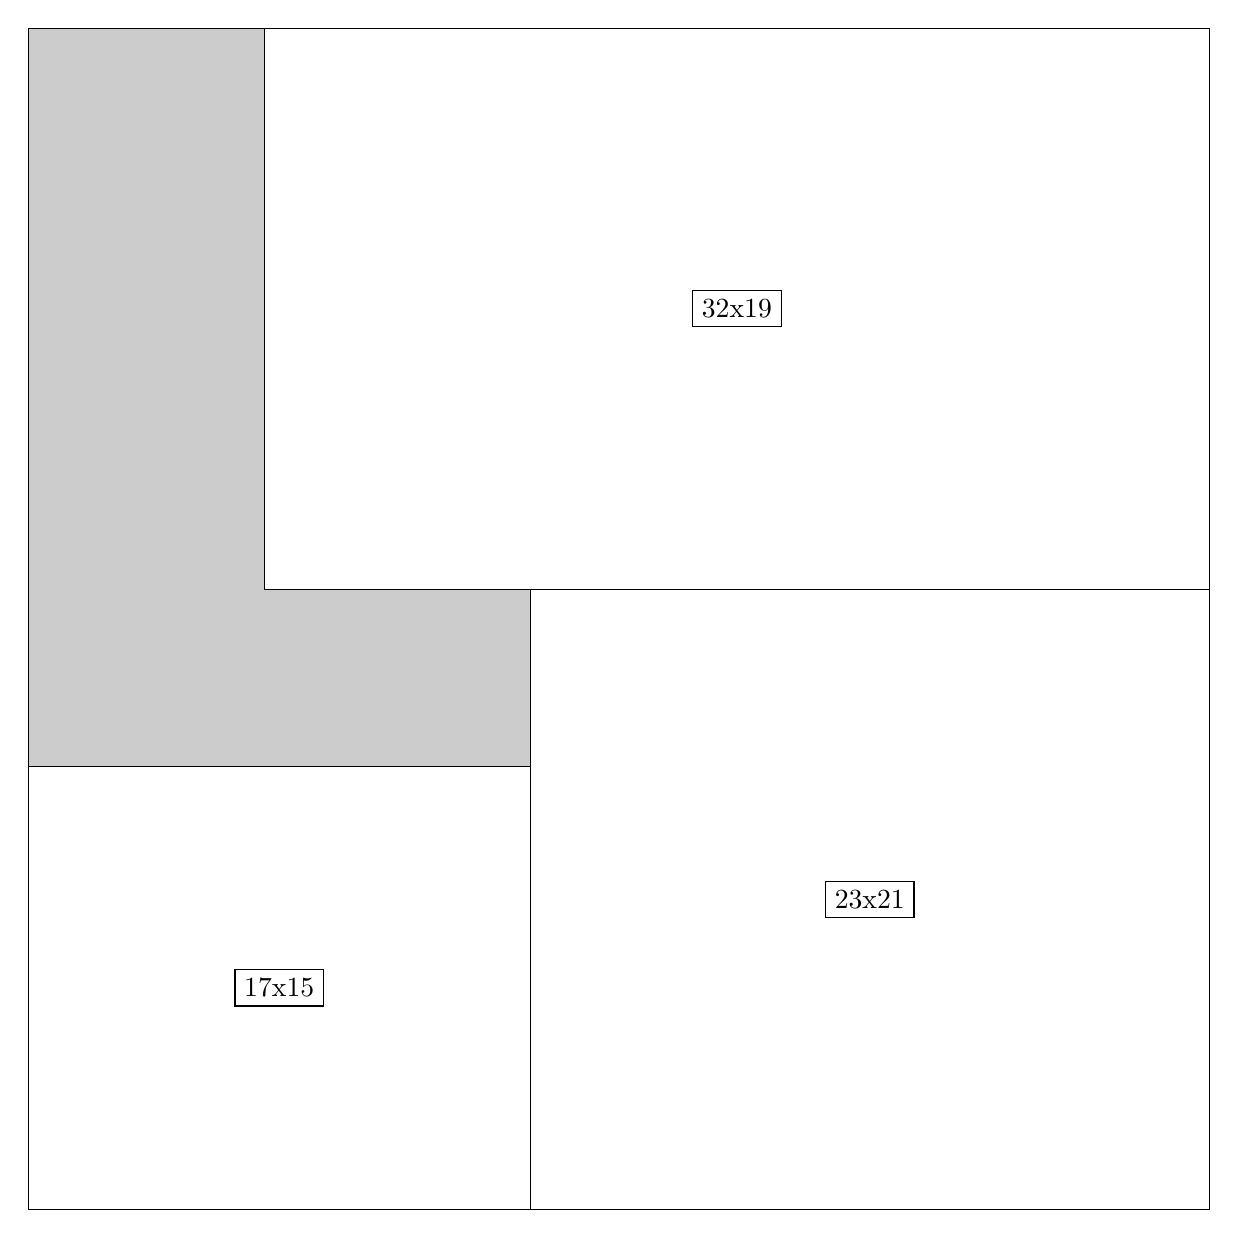
\begin{tikzpicture}[shorten >=1pt,scale=1.0,every node/.style={scale=1.0},->]
\tikzstyle{vertex}=[circle,fill=black!25,minimum size=14pt,inner sep=0pt]
\filldraw[fill=gray!40!white, draw=black] (0,0) rectangle (15.0,15.0);
\foreach \name/\x/\y/\w/\h in {23x21/6.375/0.0/8.625/7.875,17x15/0.0/0.0/6.375/5.625,32x19/3.0/7.875/12.0/7.125}
\filldraw[fill=white!40!white, draw=black] (\x,\y) rectangle node[draw] (\name) {\name} ++(\w,\h);
\end{tikzpicture}


w =23 , h =21 , x =17 , y =0 , v =483
\par
w =17 , h =15 , x =0 , y =0 , v =255
\par
w =32 , h =19 , x =8 , y =21 , v =608
\par
\newpage


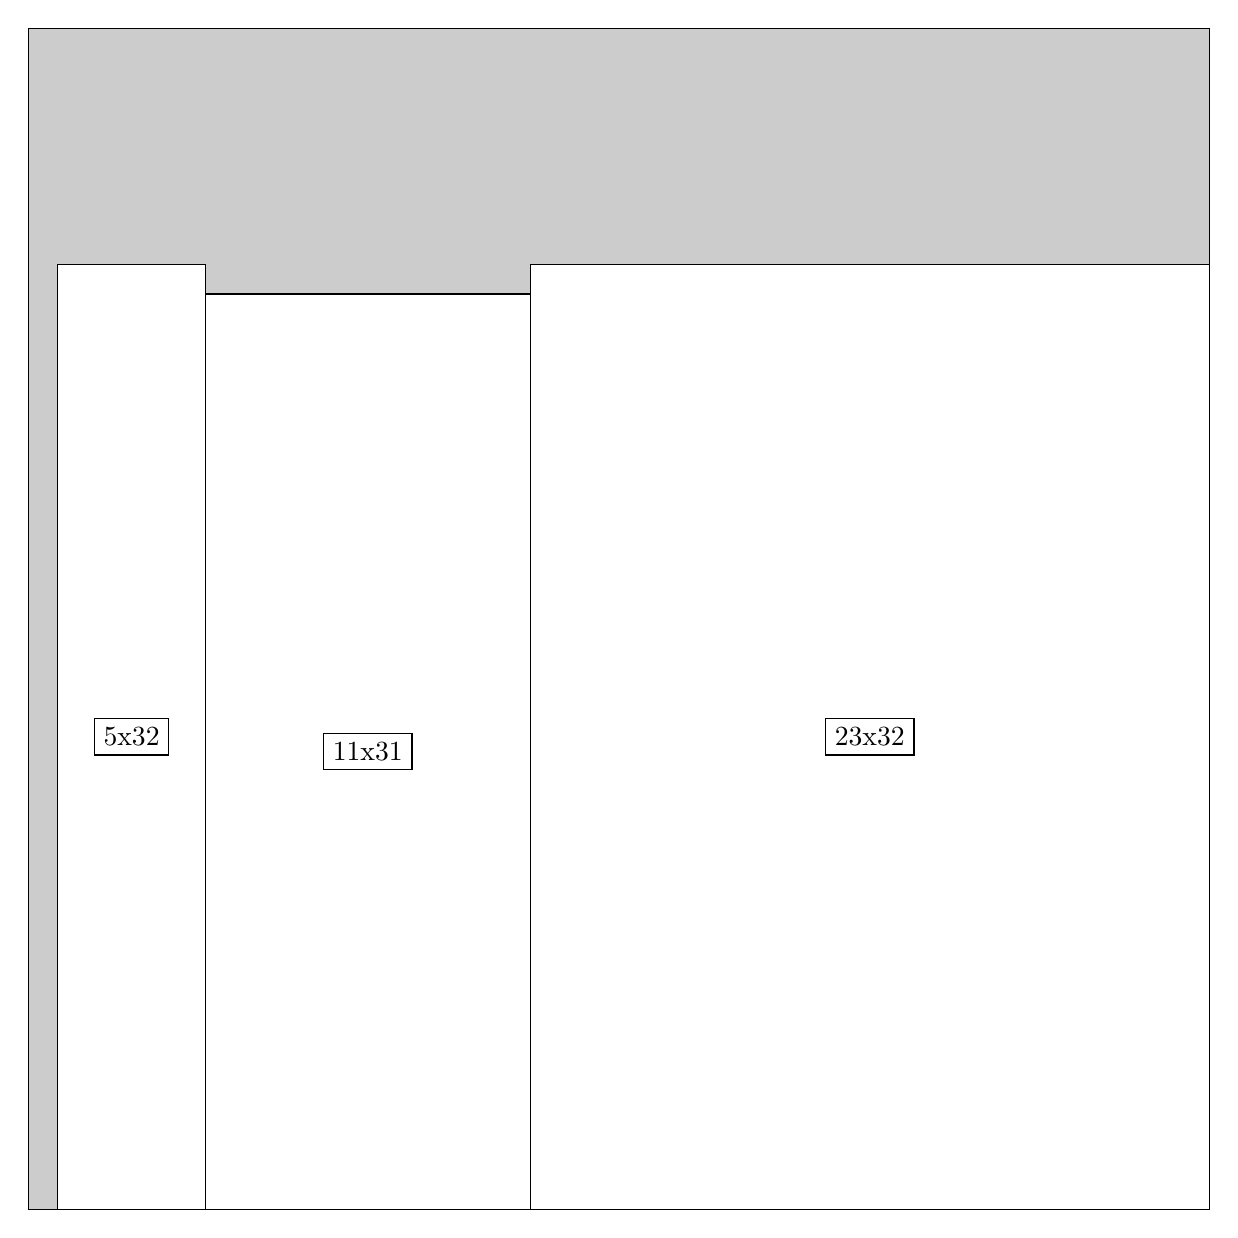
\begin{tikzpicture}[shorten >=1pt,scale=1.0,every node/.style={scale=1.0},->]
\tikzstyle{vertex}=[circle,fill=black!25,minimum size=14pt,inner sep=0pt]
\filldraw[fill=gray!40!white, draw=black] (0,0) rectangle (15.0,15.0);
\foreach \name/\x/\y/\w/\h in {23x32/6.375/0.0/8.625/12.0,11x31/2.25/0.0/4.125/11.625,5x32/0.375/0.0/1.875/12.0}
\filldraw[fill=white!40!white, draw=black] (\x,\y) rectangle node[draw] (\name) {\name} ++(\w,\h);
\end{tikzpicture}


w =23 , h =32 , x =17 , y =0 , v =736
\par
w =11 , h =31 , x =6 , y =0 , v =341
\par
w =5 , h =32 , x =1 , y =0 , v =160
\par
\newpage


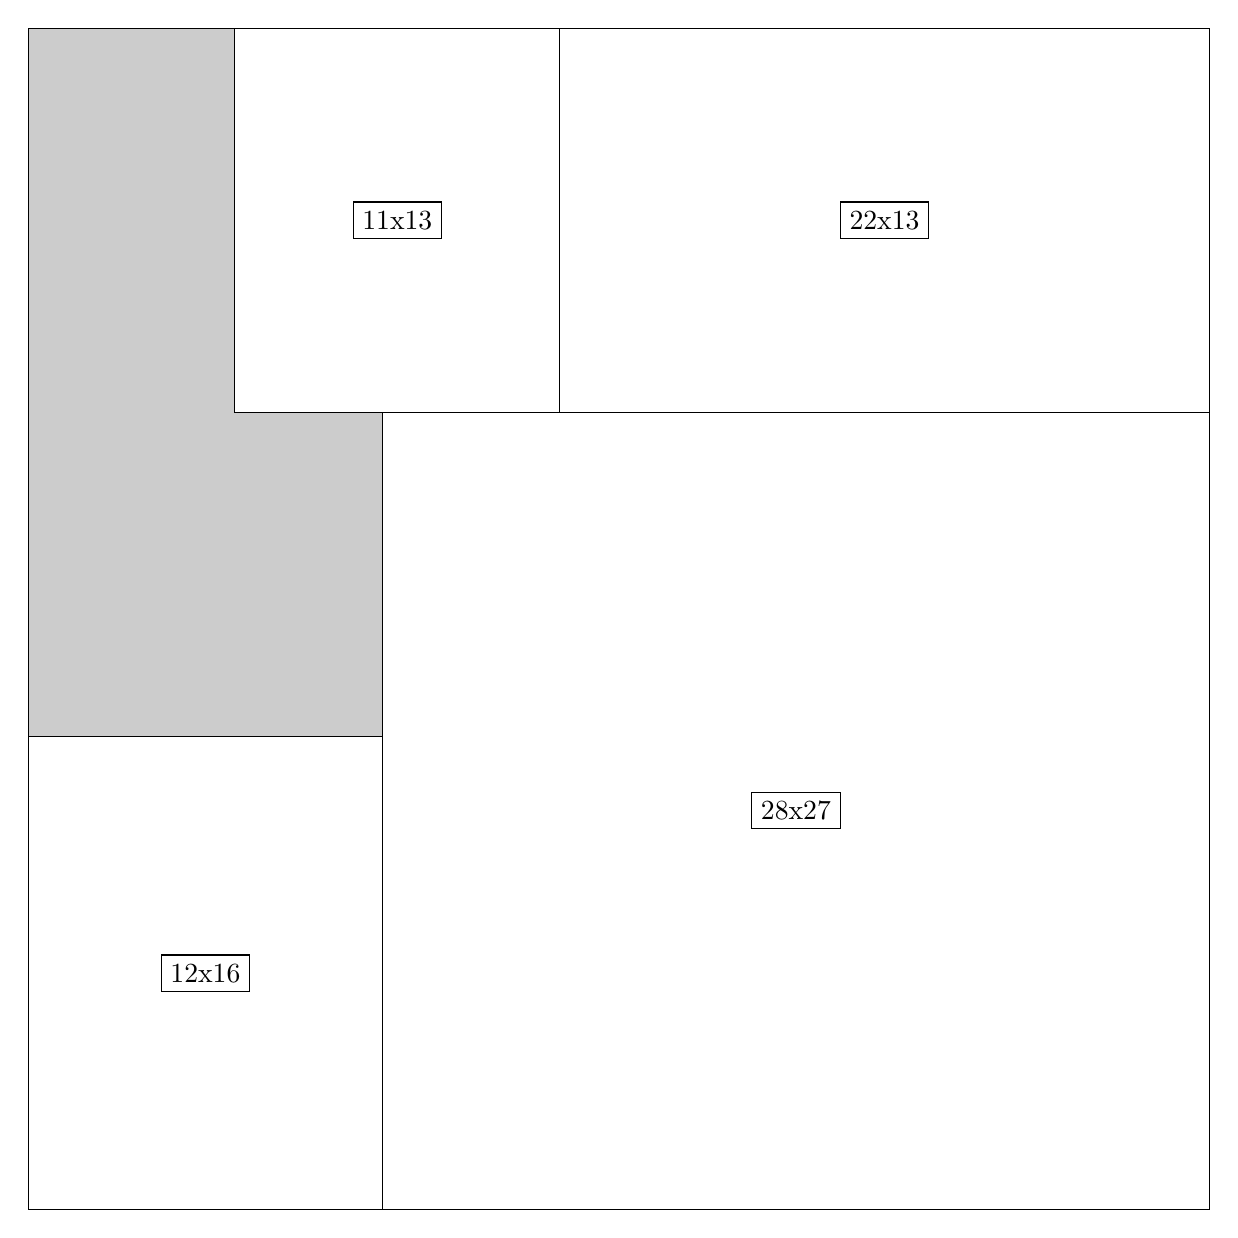
\begin{tikzpicture}[shorten >=1pt,scale=1.0,every node/.style={scale=1.0},->]
\tikzstyle{vertex}=[circle,fill=black!25,minimum size=14pt,inner sep=0pt]
\filldraw[fill=gray!40!white, draw=black] (0,0) rectangle (15.0,15.0);
\foreach \name/\x/\y/\w/\h in {28x27/4.5/0.0/10.5/10.125,12x16/0.0/0.0/4.5/6.0,22x13/6.75/10.125/8.25/4.875,11x13/2.625/10.125/4.125/4.875}
\filldraw[fill=white!40!white, draw=black] (\x,\y) rectangle node[draw] (\name) {\name} ++(\w,\h);
\end{tikzpicture}


w =28 , h =27 , x =12 , y =0 , v =756
\par
w =12 , h =16 , x =0 , y =0 , v =192
\par
w =22 , h =13 , x =18 , y =27 , v =286
\par
w =11 , h =13 , x =7 , y =27 , v =143
\par
\newpage


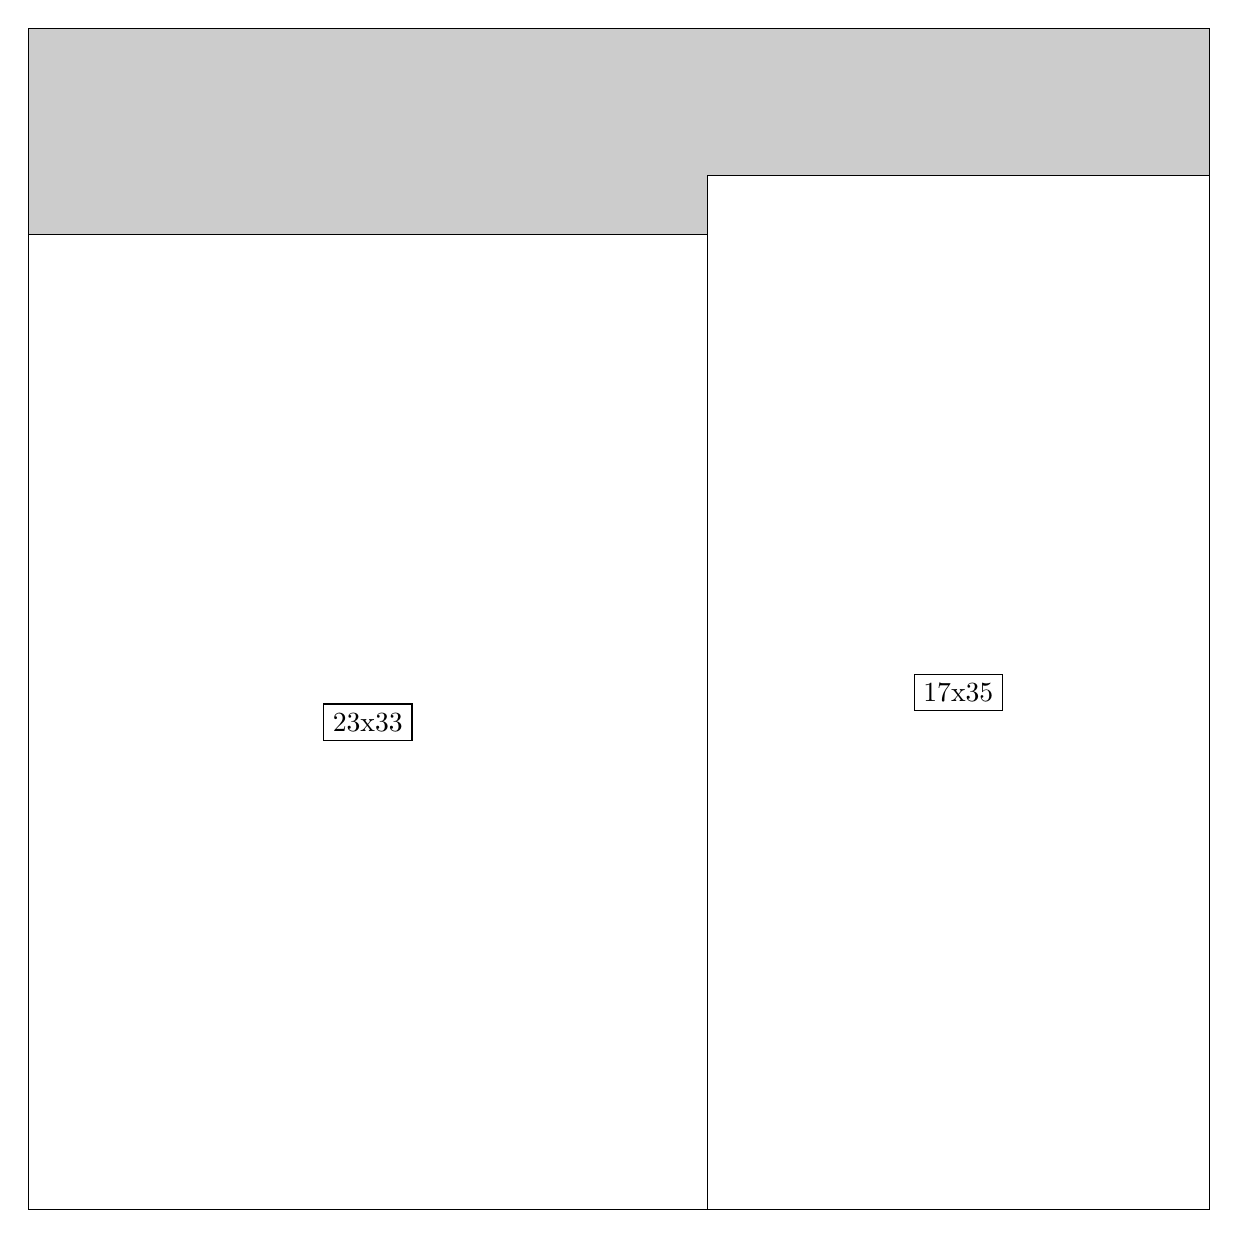
\begin{tikzpicture}[shorten >=1pt,scale=1.0,every node/.style={scale=1.0},->]
\tikzstyle{vertex}=[circle,fill=black!25,minimum size=14pt,inner sep=0pt]
\filldraw[fill=gray!40!white, draw=black] (0,0) rectangle (15.0,15.0);
\foreach \name/\x/\y/\w/\h in {17x35/8.625/0.0/6.375/13.125,23x33/0.0/0.0/8.625/12.375}
\filldraw[fill=white!40!white, draw=black] (\x,\y) rectangle node[draw] (\name) {\name} ++(\w,\h);
\end{tikzpicture}


w =17 , h =35 , x =23 , y =0 , v =595
\par
w =23 , h =33 , x =0 , y =0 , v =759
\par
\newpage


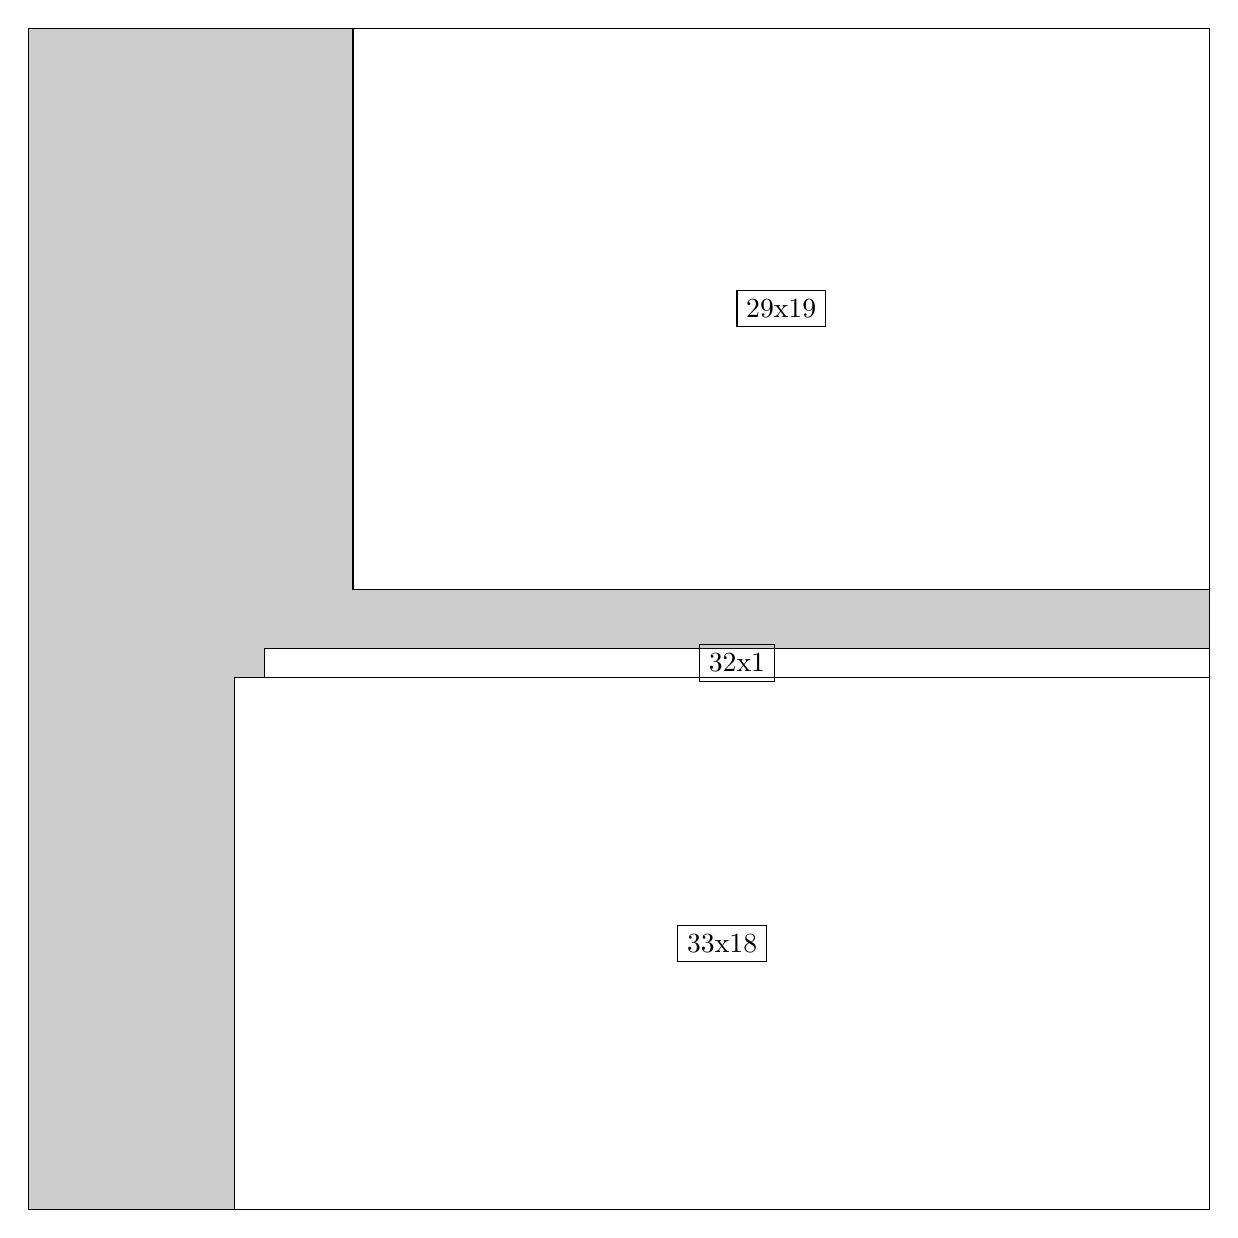
\begin{tikzpicture}[shorten >=1pt,scale=1.0,every node/.style={scale=1.0},->]
\tikzstyle{vertex}=[circle,fill=black!25,minimum size=14pt,inner sep=0pt]
\filldraw[fill=gray!40!white, draw=black] (0,0) rectangle (15.0,15.0);
\foreach \name/\x/\y/\w/\h in {33x18/2.625/0.0/12.375/6.75,32x1/3.0/6.75/12.0/0.375,29x19/4.125/7.875/10.875/7.125}
\filldraw[fill=white!40!white, draw=black] (\x,\y) rectangle node[draw] (\name) {\name} ++(\w,\h);
\end{tikzpicture}


w =33 , h =18 , x =7 , y =0 , v =594
\par
w =32 , h =1 , x =8 , y =18 , v =32
\par
w =29 , h =19 , x =11 , y =21 , v =551
\par
\newpage


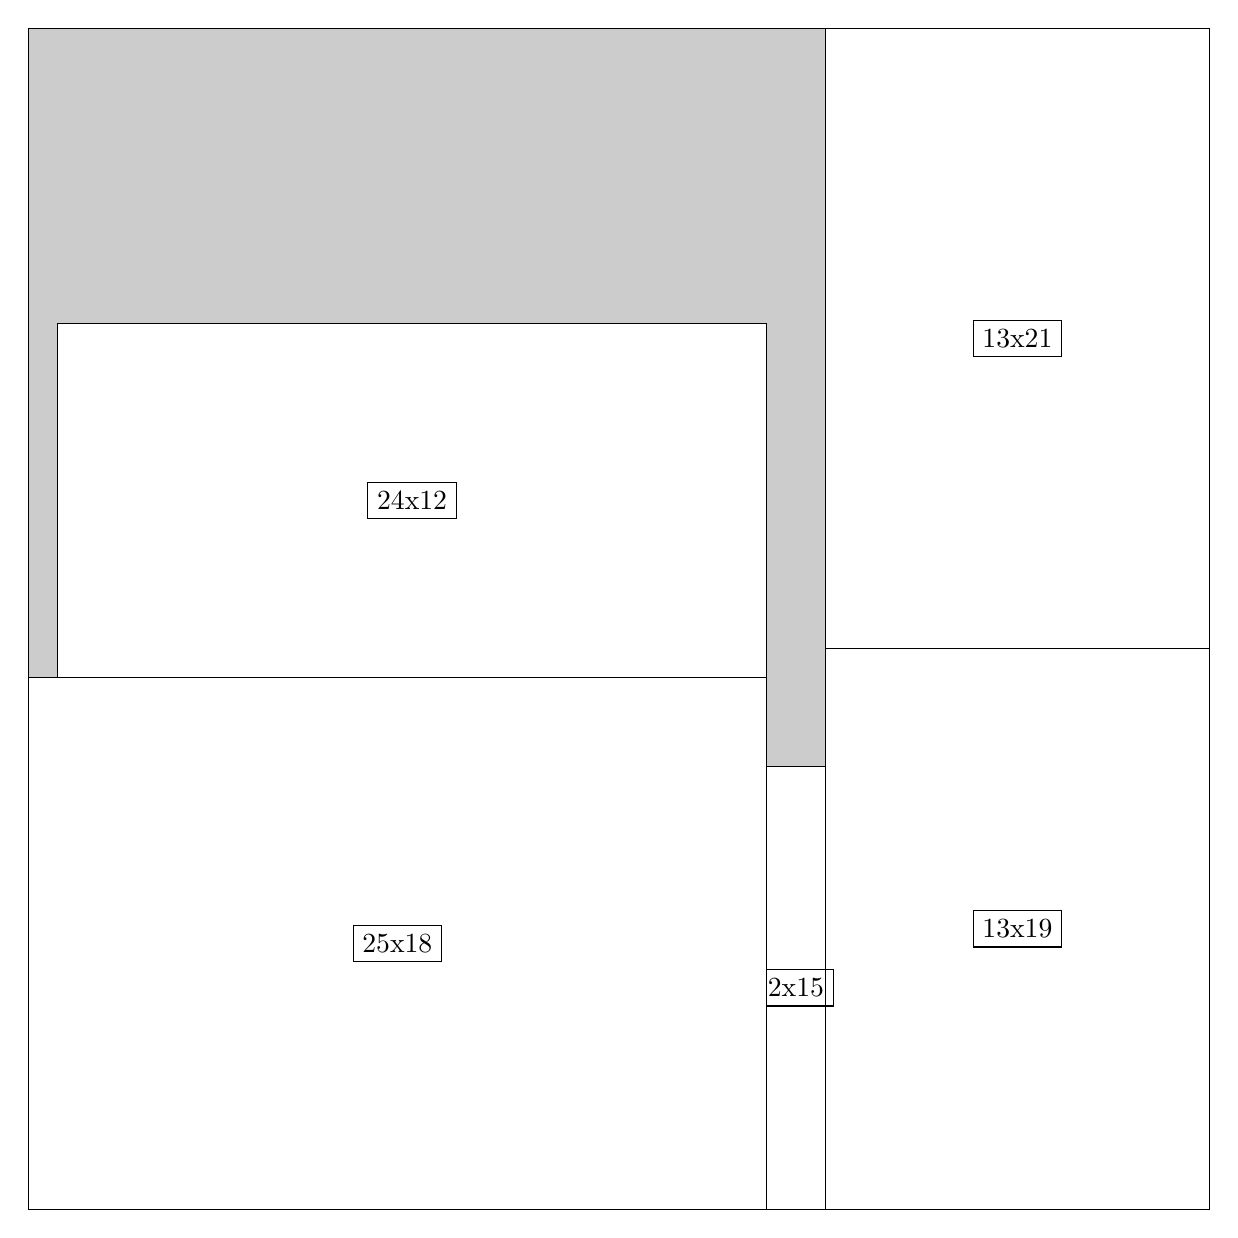
\begin{tikzpicture}[shorten >=1pt,scale=1.0,every node/.style={scale=1.0},->]
\tikzstyle{vertex}=[circle,fill=black!25,minimum size=14pt,inner sep=0pt]
\filldraw[fill=gray!40!white, draw=black] (0,0) rectangle (15.0,15.0);
\foreach \name/\x/\y/\w/\h in {13x19/10.125/0.0/4.875/7.125,2x15/9.375/0.0/0.75/5.625,13x21/10.125/7.125/4.875/7.875,25x18/0.0/0.0/9.375/6.75,24x12/0.375/6.75/9.0/4.5}
\filldraw[fill=white!40!white, draw=black] (\x,\y) rectangle node[draw] (\name) {\name} ++(\w,\h);
\end{tikzpicture}


w =13 , h =19 , x =27 , y =0 , v =247
\par
w =2 , h =15 , x =25 , y =0 , v =30
\par
w =13 , h =21 , x =27 , y =19 , v =273
\par
w =25 , h =18 , x =0 , y =0 , v =450
\par
w =24 , h =12 , x =1 , y =18 , v =288
\par
\newpage


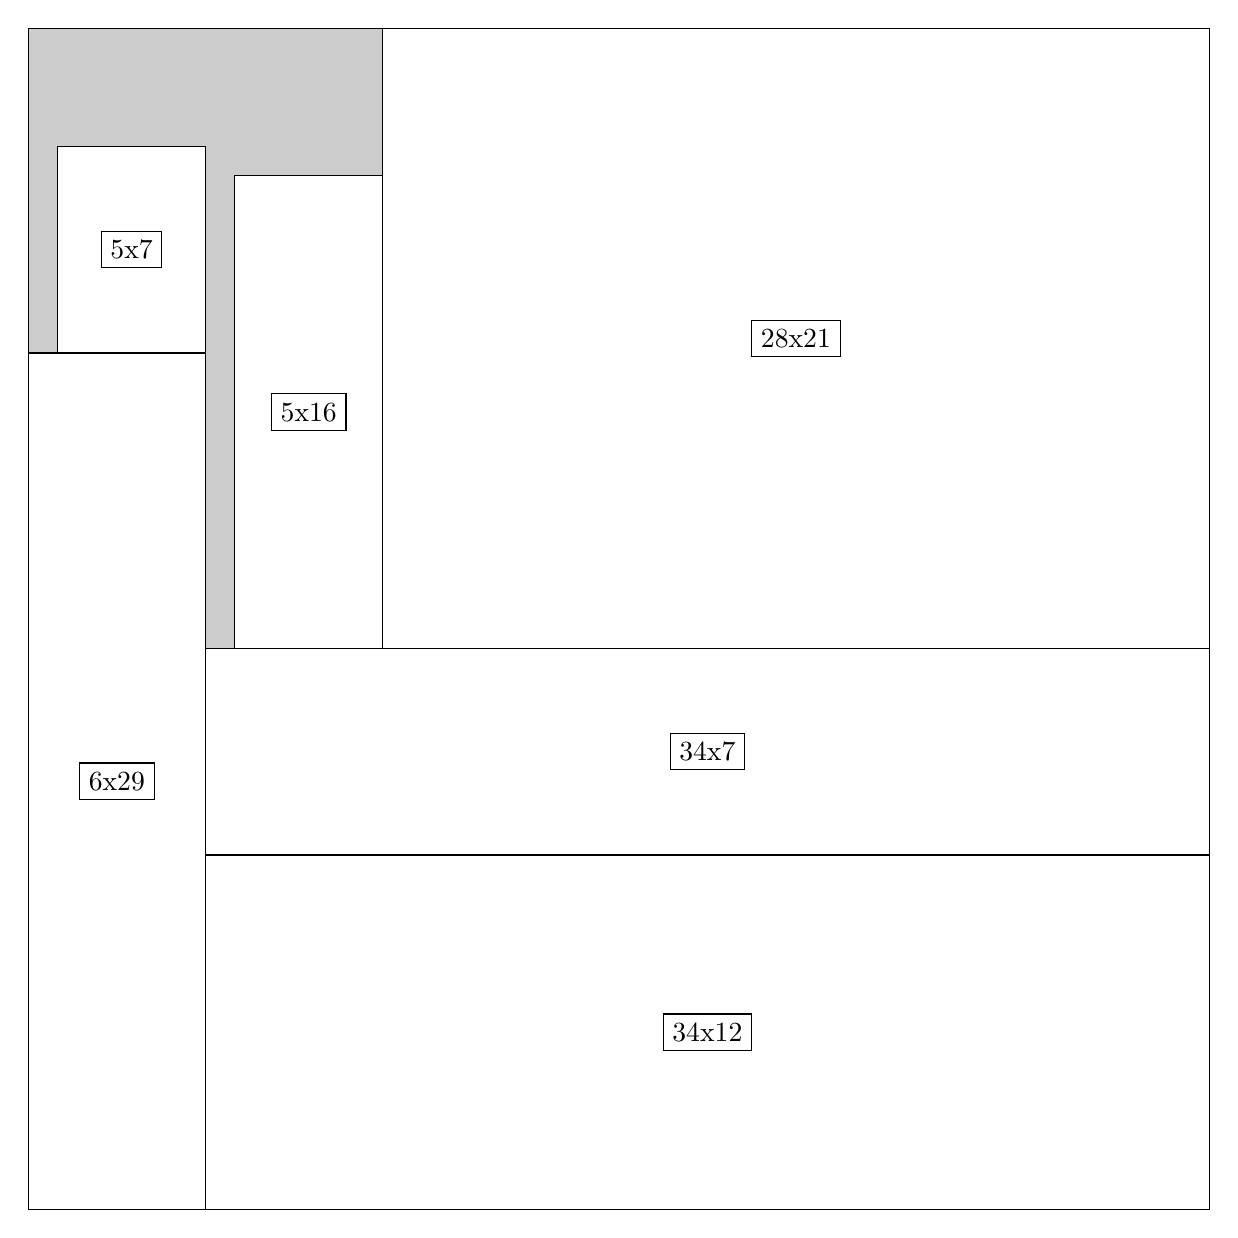
\begin{tikzpicture}[shorten >=1pt,scale=1.0,every node/.style={scale=1.0},->]
\tikzstyle{vertex}=[circle,fill=black!25,minimum size=14pt,inner sep=0pt]
\filldraw[fill=gray!40!white, draw=black] (0,0) rectangle (15.0,15.0);
\foreach \name/\x/\y/\w/\h in {34x12/2.25/0.0/12.75/4.5,34x7/2.25/4.5/12.75/2.625,28x21/4.5/7.125/10.5/7.875,5x16/2.625/7.125/1.875/6.0,6x29/0.0/0.0/2.25/10.875,5x7/0.375/10.875/1.875/2.625}
\filldraw[fill=white!40!white, draw=black] (\x,\y) rectangle node[draw] (\name) {\name} ++(\w,\h);
\end{tikzpicture}


w =34 , h =12 , x =6 , y =0 , v =408
\par
w =34 , h =7 , x =6 , y =12 , v =238
\par
w =28 , h =21 , x =12 , y =19 , v =588
\par
w =5 , h =16 , x =7 , y =19 , v =80
\par
w =6 , h =29 , x =0 , y =0 , v =174
\par
w =5 , h =7 , x =1 , y =29 , v =35
\par
\newpage


\end{document}